%%=======================================
%  XSYU Bachelor Thesis v 0.1b
%  Originaly by: Tsao Yu
%  tsaoyu@tsaoyu.com
%  Modified by: Liumei Zhang
%  zhangliumei@xsyu.edu.cn
%  Last Modify Date Jun.14,2016
%%=======================================

\documentclass[cs4size,a4paper]{ctexart}
\usepackage{xeCJK}
%\usepackage{CJK}
\usepackage[subfigure]{tocloft}%章节总标题加点
\renewcommand{\cftsecleader}{\cftdotfill{\cftdotsep}}%章节总标题加点

%==================== 数学符号公式 ============
\usepackage{amsmath}                 % AMS LaTeX宏包
\usepackage{amssymb}                % 用来排版漂亮的数学公式
%\usepackage{amsbsy}
\usepackage[style=1]{mdframed}
\usepackage{amsthm}
\usepackage{amsfonts}
\usepackage{mathrsfs}                % 英文花体字 体
\usepackage{bm}                      % 数学公式中的黑斜体
\usepackage{bbding,manfnt}           % 一些图标,如 \dbend
\usepackage{lettrine}
\usepackage{mathtools}
     % 首字下沉,命令\lettrine
\def\attention{\lettrine[lines=2,lraise=0,nindent=0em]{\large\textdbend\hspace{1mm}}{}}
\usepackage{longtable}
\usepackage[toc,page]{appendix}
\usepackage{geometry}                % 页边距调整
\geometry{top=3.0cm,bottom=2.7cm,left=3cm,right=2.5cm}
%\usepackage{caption2}               % 浮动图形和表格标题样式
\DeclareMathOperator*{\argmax}{arg\,max}
\DeclareMathOperator*{\argmin}{arg\,min}
%====================公式按章编号==========================
\numberwithin{equation}{section}
\numberwithin{table}{section}
\numberwithin{figure}{section}

%===================表格=================================
\usepackage{booktabs}
\newcommand{\tabincel}[2]{\begin{tabular}{@{}#1@{}}#2\end{tabular}}
\usepackage{rotating}
\usepackage{tabularx}
\usepackage{multirow}
\usepackage{longtable,lscape}

%==================图片=================================
%\usepackage[font=small,labelfont=bf]{caption}
\usepackage[font=small,labelfont=bf]{caption}

%================= 基本格式预置 ===========================

\usepackage{fancyhdr}
\pagestyle{fancy}
\fancyhf{}
\fancyhead[C]{\zihao{5}  \songti 西安石油大学硕士学位论文 }
\fancyfoot[C]{~\zihao{5} \thepage~}
\renewcommand{\headrulewidth}{0.65pt}
\CTEXsetup[format={\centering\bfseries\zihao{3}\songti},name={, }]{section}
%\CTEXsetup[format={\centering\bfseries\zihao{-2}},name={第, 章}]{section}
\CTEXsetup[format={\bfseries\zihao{4}\songti}]{subsection}
\CTEXsetup[format={\bfseries\zihao{-4}\songti}]{subsubsection}
\newcommand{\upcite}[1]{\textsuperscript{\textsuperscript{\cite{#1}}}}%上标引用格式
\renewcommand{\cftsecleader}{\cftdotfill{\cftdotsep}}
\usepackage[font=small,labelfont=bf, textfont=bf]{caption}
%================== 图形支持宏包 =========================
\usepackage{subfigure}
\usepackage{graphicx}                % 嵌入png图像
\usepackage{color,xcolor}            % 支持彩色文本、底色、文本框等
\usepackage{pifont}                    %支持圈数字 %\ding{number}
\usepackage{hyperref}                % 交叉引用
\usepackage{caption}
\captionsetup{figurewithin=section}
%==================== 源码和流程图 =====================
\usepackage{listings}                % 粘贴源代码
\usepackage{tikz}
\usepackage{tikz-3dplot}
\usetikzlibrary{shapes,arrows,positioning}

%==================== 字体设置区 ============
%\setCJKmainfont[BoldFont=宋体-简 粗体,ItalicFont=宋体-简 常规体]{宋体-简 常规体}
\setCJKmainfont{SimSun}
%\setCJKsansfont[BoldFont=宋体-简 常规体]{宋体-简 常规体}
\setCJKsansfont{SimSun}
\setCJKmonofont{SimSun}
\setmainfont{Times New Roman}
%==================== 自定义包 =======================
%===================  定理类环境定义 ===================
\newtheorem{example}{例}              % 整体编号
\newtheorem{algorithm}{算法}
\newtheorem{theorem}{定理}            % 按 section 编号
\newtheorem{definition}{定义}
\newtheorem{axiom}{公理}
\newtheorem{property}{性质}
\newtheorem{proposition}{命题}
\newtheorem{lemma}{引理}
\newtheorem{corollary}{推论}
\newtheorem{remark}{注解}
\newtheorem{condition}{条件}
\newtheorem{conclusion}{结论}
\newtheorem{assumption}{假设}
\usepackage{enumitem}
%===================   正文开始    ===================
\begin{document}
	\bibliographystyle{gbt7714-2005}     %论文引用格式
	%==================重定义 ===================
\renewcommand{\contentsname}{\hspace*{\fill}目\quad 录\hspace*{\fill}}
\renewcommand{\abstractname}{摘要}
\renewcommand{\refname}{参考文献}
\renewcommand{\indexname}{索引}
\renewcommand\thefigure{\thesection-\arabic{figure}}
\renewcommand{\figurename}{图}
\renewcommand\thetable{\thesection-\arabic{table}}
\renewcommand{\tablename}{表}
\renewcommand{\appendixname}{附录}
\renewcommand{\proofname}{证明}
\renewcommand{\algorithm}{算法}
%\renewcommand{\labelenumi}{(\arabic{enumi})}
%============== 自定义 ===================
%\setlength{\parindent}{1em}
\fancypagestyle{plain}{
	\pagestyle{fancy}
}%目录页加页眉

%============== 封皮和前言 =================
%%===============  封面  =================
\smallskip
\vspace*{2.0cm}
\begin{center}
\begin{figure}[!th]
\centering

\includegraphics[width=0.3\linewidth]{figure/SchoolName}
\end{figure}

\vspace*{1.0cm}{\zihao{-1} \textbf{\songti{} 硕士学位论文}} \\
\vspace*{9.0cm} \songti{}
% 创建表内换行
\newcommand{\tabincell}[2]{\begin{tabular}{@{}#1@{}}#2\end{tabular}}
\begin{tabular}{lc}
  \zihao{3} \textbf{题\hspace{\fill}目:} &
  \underline{\makebox[7cm][c]{\tabincell{c}{\zihao{3}图像内容识别技术在\\}}} \\
  \zihao{3} \textbf{\hspace{\fill}} &
  \underline{\makebox[7cm][c]{\tabincell{c}{\zihao{3}对比挖掘中的应用研究\\}}}\\
  \zihao{3}\textbf{作者姓名:} &
  \underline{\makebox[7cm][c]{\zihao{4}任萌}} \\
\\
  \zihao{-3}\textbf{导师姓名、职称:} &
  \underline{\makebox[7cm][c]{\zihao{4}计算机学院}} \\
\\
  \zihao{3}\textbf{学科(专业)名称:} &
  \underline{\makebox[7cm][c]{\zihao{4}计算机应用技术}} \\
\\
  \zihao{3}\textbf{提交论文日期:} &
  \underline{\makebox[7cm][c]{\zihao{4}2020年6月1日}} \\
\\
\end{tabular}
\end{center}
\thispagestyle{empty}
\clearpage

\pagestyle{plain}          %不带页眉横线
%\thispagestyle{empty}
\fancyhead[C]{\zihao{5}  \songti 摘\hspace{1em}要}
\section*{\zihao{-3} \centering 情感挖掘技术在证券分析中的应用研究}
%\vspace{0.5cm}

\noindent
\section*{\zihao{-3} \centering \textbf{摘\hspace{1em}要}}

技术的快速发展改变了投资者社交和购买决策的动力。过去十年中,在线评论的数量迅速增长,导致投资者群体在购买决策过程中承担了不成比例的重量。对于运营商试图将评论纳入分析中来说,大量的评论可能是一项艰巨的任务。情感分析允许以相对容易且时间敏感的方式处理大量消费者评论。这些评论中包含的信息,情感分数,与其他消费者在做出购买决定之前从其他消费者那里收集到的情感相同。为了证明这些评论的重要性,本研究将试图使用消费者评论的情绪作为主要预测因素来股票价格的方向变化。本次研究从雪球网爬取的20只股票的历史价格信息和对应的投资者评论信息出发。对投资者的评论进行情感分析后采用MIC(最大信息系数)度量价格趋势和投资者态度之间的相关性。我们得出在线评论的消费者情绪将对股价的未来方向性趋势具有重要意义。

\vspace{0.5cm}
\noindent
\textbf{关键词:}情感挖掘 ;在线评论;数据处理;证券分析;MIC
%\addcontentsline{toc}{section}{摘要}%摘要是否包括进目录中

\clearpage

%\thispagestyle{empty}
\fancyhead[C]{\zihao{5}  \songti Abstract}
\section*{\songti\zihao{-3} \centering Research on the application of sentiment mining technology in stock analysis}

\section*{\zihao{-3} \textbf{Abstract}}
   %用了Times New Roman字体来美化观感
\noindent
The rapid development of technology has changed the dynamics of social and purchasing decisions for investors. The number of online reviews has grown rapidly over the past decade, leading to a disproportionate share of the weight of the investor community in the purchase decision process. A lot of comments can be a daunting task for operators trying to incorporate comments into their analysis. Affective analysis allows for a relatively easy and time-sensitive way to handle a large number of consumer reviews. These comments contain information about the same emotional score that other consumers collected from other consumers before making a purchase decision. To demonstrate the importance of these reviews, this study will attempt to use the sentiment of consumer commentary as a major predictor of the direction of stock price changes. This study starts with the historical price information of 20 stocks crawled by the snowball net and the corresponding investor's comment information. The relationship between the price trend and the investor's attitude is measured by the MIC (Maximum Information Coefficient) after the emotional analysis of the investor's comments. The consumer sentiment that we have come up with online commentary will be of great significance to the future directional trend of stock price.

\vspace{0.5cm}
\noindent
\textbf{Keywords: }Sentiment Analysis;Online Review; Data Processing; Stock Analysis; MIC
%\addcontentsline{toc}{section}{Abstract}%英文摘要是否包括进入目录


\pagenumbering{Roman}
\renewcommand{\cftdot}{.}

%\thispagestyle{plain}%页眉横线,标题
\fancyhead[C]{\zihao{5}  \songti \textbf{目\hspace{1em}录}}
\tableofcontents
\newpage

%============== 论文正文   =================
\pagestyle{plain}

\pagenumbering{arabic}

\fancyhead[C]{\zihao{5}  \songti 西安石油大学硕士学位论文 }

\section{绪论}

\subsection{研究背景及意义}

\subsubsection{研究背景}


参考文献引用:~\upcite{huang2008stock}


\subsubsection{研究意义}



\subsection{研究目的}



\subsection{本文的主要内容}
 

\subsection{本文的组织结构}

在第~\ref{数据采集}节,将介绍股票评论文本的采集和储存。
在第~\ref{评论情感分析}节将介绍评论的情感分析,包括原理和所采用的技术。
在第~\ref{股票影响分析}节,将对评论的情感对股票的价格的影响进行分析及结论。
最后在第~\ref{总结}节总结本文。

\section{相关工作}~\label{related-work}
\subsection{用户评论}



\subsection{文本情感分析}



\subsubsection{基于词典的分析}

基于词典的方法使用具有预先分配给它们的值的词的词典来确定价态取向\upcite{chiu2015opinion}。这个过程涉及手动创建要识别的术语,并且可以被认为是一种监督方法,并且是以该领域为基础构建的\upcite{taboada2011lexicon}。
这种方法的一个主要缺点是,词典的功效在用于不同的领域时会迅速减少,因为术语的转变以及可能代表积极情绪的词语现在被认为是负面的。这方面的一个例子是“按摩很慢并需要花费数小时”的评论通常被认为是一种积极的情绪,因为按摩的目的是鼓励放松,并最大限度地延长在该州的时间花费。
相反,“晚餐服务很慢,需要花费数小时”传达出不同的情绪,因为餐厅服务的预期是及时的。
尽管这两个例子都在酒店业,并且甚至可能发生在同一个度假胜地,但如果分析工作正在进行中,将“慢”一词包含在语义词典中作为负面情绪可能会产生不利影响一个文件,甚至是句子层面的分析。然而,基于词典的方法学的使用确实具有优势。包含特定“俚语”或本地方言独特性的能力可以被更仔细地考虑。这包括所描述项目的特定属性,并且可能包括在单独的上下文中可能构成乱码或其他不相关的项目\upcite{taboada2011lexicon}。


\subsubsection{文本分类}

传统上,在文档层面,只使用了两个层次的分类,情绪可能是正面的或负面的\upcite{liu2012sentiment}。文件的这种广泛的分类,特别是在消费者评论的情况下,可以通过分配给该产品的总评分轻易识别。
Pang,Lee等人\upcite{pang2002thumbs}研究人类直觉或机器学习的最佳过程是否是人类直觉或机器学习。人类主题根据直观的单词列表将电影评论分为正面,负面或“领带”。领带类别是当评论被同等评价为正面和负面时。人类的直觉方法导致了中等的准确性(58-64%),但非常高的平均率(39-75%)。通过使用由数据中使用的最高频率词构建的语料库并使用该统计构建列表对准确率(69%)的准确率超过直观列表并降低整体联系率(16% )(Pang等,2002)。然后他们测试了三种不同的基于机器的方法,NaïveBayes,最大熵分类和支持向量机,并将这些人类分类评分作为基于机器的算法挑战者的支持者。他们的测试框架涉及一组预定义的$n$元组的分类,其中每个文档$d$是$n_i(d)$的向量,$n_i(d)$是$f_i$在文档中出现的次数。

Pang et al\upcite{pang2002thumbs}对电影评论的分析使用unigrams和bi-gram有助于取得最佳效果。即使朴素贝叶斯理论上违背了条件独立假设,双重克的增加比单独使用单数频率的效果要好,但是比单一格的存在要差0.4%。这三种方法都远远超过了控制方法中设定的人类分类基准,并且这三种方法的准确率接近,支持向量机在朴素贝叶斯上略有优势(Pang et al。,2002)。Pang等人\upcite{pang2002thumbs} 确实注意到,情感识别不如使用相同方法的主题分类准确,并且认为这可能是由于评论中使用的语言的性质以及在上下文中可以构建的矛盾意义。作为一个例子,一位评论员说,有问题的电影“是一部非常糟糕的电影......地狱的第九层。情节很混乱,很糟糕。但我喜欢它“。这种类型的评论很容易被人类分类器确定为正面,但基于机器的算法会识别大量的底片,并可能对其进行错误分类。为此,作者建议确定句子是否集中在正确的主题上,因为“整体不一定是各部分的总和”\upcite{pang2002thumbs}。

文档级审查的方法足以提供对产品情感的总体概念,但其限制是它无法提供有关产品方面的细节,也不能轻易地应用到产品的讨论区 话题可能暗示或转移。 尽管Liu\upcite{liu2012sentiment}指出:“在线评论不需要情感分类,因为几乎所有的评论都已经有用户分配的星级”,随后的研究表明评论的内容可能比最初的影响力更大,因为可能恶魔 往往隐藏在细节中。

\subsubsection{基于句子的情感分析}

基于句子的情感分析在许多方面与文档级分析类似\upcite{liu2012sentiment}。 这是由于句子的性质,这是完整的想法,基本上只是从分析的角度来看短文本。 基于句子情感分析的过程与基于文档分析的过程类似,但更侧重于客观与主观陈述的区别。

一般来说,评论是由多个单独文本的简单句子组成。 然而,正如Liu(2012)所指出的那样,评论具有已知的整体情绪,可能不能反映评论中包含的具体情绪。 判断情绪分析可能会与评论者留下的整体评分发生冲突,或评论的各个部分可能会发生冲突。 虽然Philander等人\upcite{philander2016twitter}使用基于文档的分类方法,但他们的兴趣领域是Twitter。 Twitter将任何“推特”限制为最多140个字符。 这个限制限制了可以形成的句子的数量,因为三个句子往往将超过140个字符的限制。

相比之下,在线评论网站并没有对评论的长度做出这样的限制\upcite{sparks2011impact}。有些网站对评论的长度没有任何限制,导致网上评论在情感深度和篇幅上都有所不同。然而,在句子层面上分析这一审查并与文件层次和邻近句子进行比较会产生更高的准确性\upcite{mcdonald2007structured}。 在McDonald的研究中,他们提出通过评估文档评估中的句子可以产生更准确的结果。 这超出了文档级别分类的准确性,但他们表明,在评估每个句子并不取决于前面的句子情绪,产生了最不准确的结果\upcite{mcdonald2007structured}。分析的准确性增加是通过使用嵌套分类和创建句子分类与整体文档分类的约束条件来实现的。也就是说,每个句子都是从整个文档的极性位置开始评估的,并且还与每个句子进行比较。 虽然\upcite{liu2012sentiment}建议仔细评估句子以从基于主观和情感的或基于客观情绪的角度确定客观的基于非情绪的陈述,但Mcdonald等人评估的客观陈述是中性的,因此没有 影响整体分类。

\section{数据采集}~\label{数据采集}

\begin{figure}[thbp!]
  \centering
  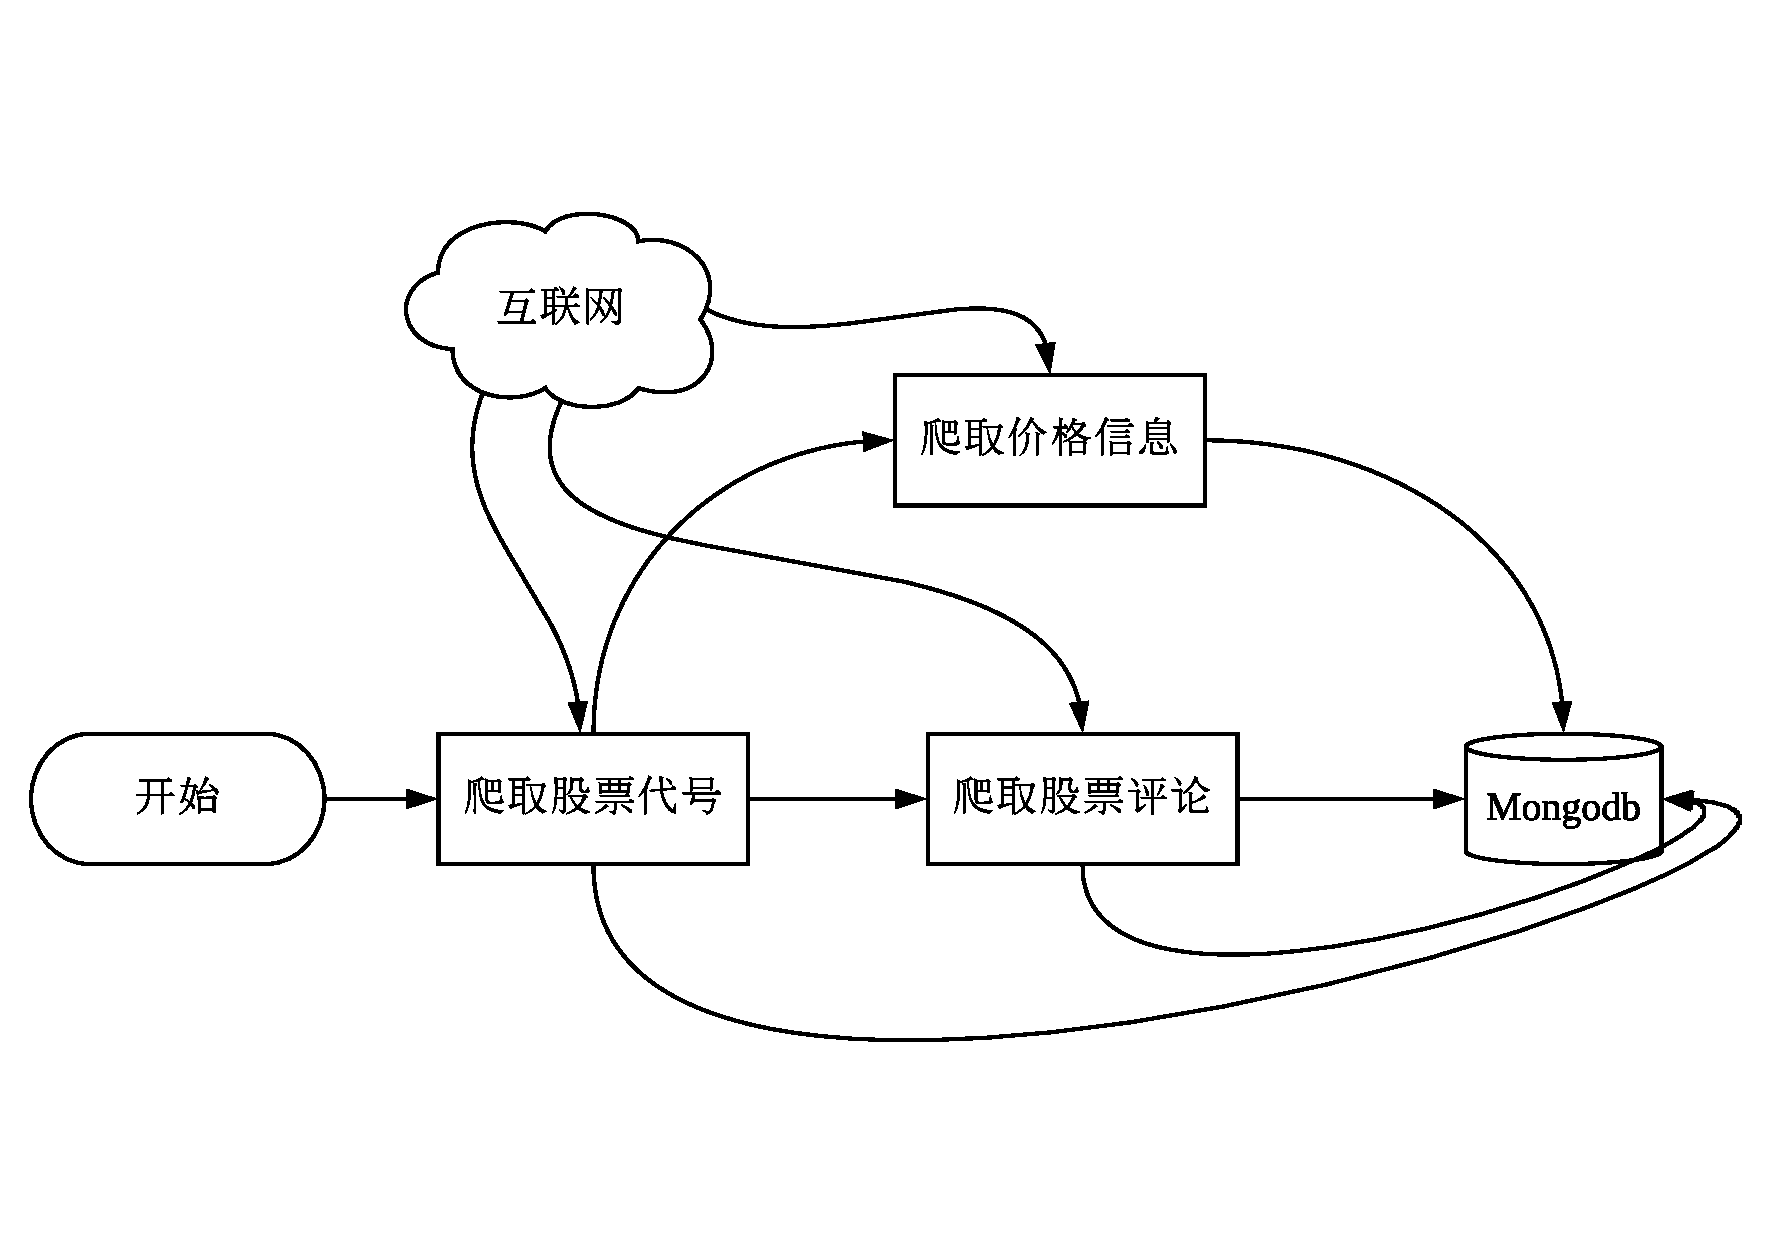
\includegraphics[width=0.8\textwidth]{figure/spiderProcess.pdf}
  \caption{爬虫流程}\label{fig:spiderPrecess}
\end{figure}

\subsection{数据储存}

\subsubsection{NoSQL}

从网络上抓取的数据需要存储起来方便之后的后续分析和处理。一般存储数据的方式一种是为存储为可供程序读取得文件如csv,json等,另一种为直接写入数据库。
写入数据库的好处是保证数据存储和应用程序分离,保证数据的完整性和安全性并且具有高效自同步等特性。本文将采用数据库存取的方式管理数据。

由于网路数据的复杂和非结构化等特征,本文所采用的数据库为NoSQL。 NoSQL最初是指“非SQL”或“非关系型”)\upcite{Nosql}数据库,它提供了一种存储和检索数据的机制,这种机制的建模方式不是关系数据库中使用的表格关系。 这些数据库自20世纪60年代后期就已存在,但直到二十一世纪早期受欢迎程度激增之后才获得“NoSQL” 绰号,由Web 2.0公司的需求触发,如Facebook,Google和Amazon\upcite{AamzonNosql}。NoSQL数据库越来越多地用于大数据和实时Web应用程序。 NoSQL系统有时也被称为“不仅仅是SQL”,以强调它们可以支持类似SQL的查询语言。

NoSQL数据库可以有很多分类方法,每种数据库都有不同的类别和子类别,其中一些类别重叠。 下面是数据模型基本可分为:列储存 、 文件储存、键值对、 图储存 和多模型储存这5种。

\subsubsection{MongoDB}

MongoDB正是一个免费且开放源码的跨平台采用 文件储存的NoSQL数据库程序。
并使用类似JSON的文档和模式。它由MongoDB Inc.开发,并且在GNU Affero General Public License和Apache License的组合下发布。\upcite{MongoDb}

文件存储的核心概念是“文件”的概念。
虽然每个面向文档的数据库实现在这个定义的细节上有所不同,但总的来说,它们都假定文档以某些标准格式或编码封装和编码数据(或信息)。正在使用的编码包括XML,YAML和JSON以及像BSON这样的二进制形式。文档通过代表该文档的唯一密钥在数据库中寻址。面向文档数据库的其他定义特征之一是,除了通过键值存储执行密钥查找之外,数据库还提供API或查询语言,以根据其内容检索文档。
不同的实现提供了不同的组织和/或分组文档的方式:

MongoDB采用集合的方式组织和分组文档。 与关系数据库相比,集合可以被认为类似于类似于记录的表和文档。但它们不同之处在于:表中的每个记录具有相同的字段序列,而集合中的文档可能具有完全不同的字段。

MongoDB支持字段,范围查询,正则表达式搜索。查询可以返回文档的特定字段,还可以包含用户定义的JavaScript 函数。
查询也可以配置为返回给定大小的结果的随机样本。
所以 MongoDB是一个存取网络数据的非常好的选择。
在本研究中,分别将爬取的股票代号、股票价格和股票评论建立了相应的集合保存在MongoDB下。共爬取 5219支股票,针对这些股票代号共抓取 306107条历史价格条目。由于考虑到大规模的爬取评论会给网站带来很大的压力。在本研究中选取了评论稳定价格波动平稳的20 支股票共抓取了3687条评论。
抓取的评论数据如图~\ref{fig:comment}所示。

\begin{figure}
  \centering
  \includegraphics[width=\textwidth]{figure/comment.png}
  \caption{评论数据示例}\label{fig:comment}
\end{figure}

\subsection{文本数据预处理}

从论坛爬取的数据大多含有噪音的,非结构化的数据文本,需要对这些数据进行一系列预处理才能进行情感分析,文本处理的流程图如图~\ref{fig:textPrecess} 所示。
\begin{figure}
  \centering
  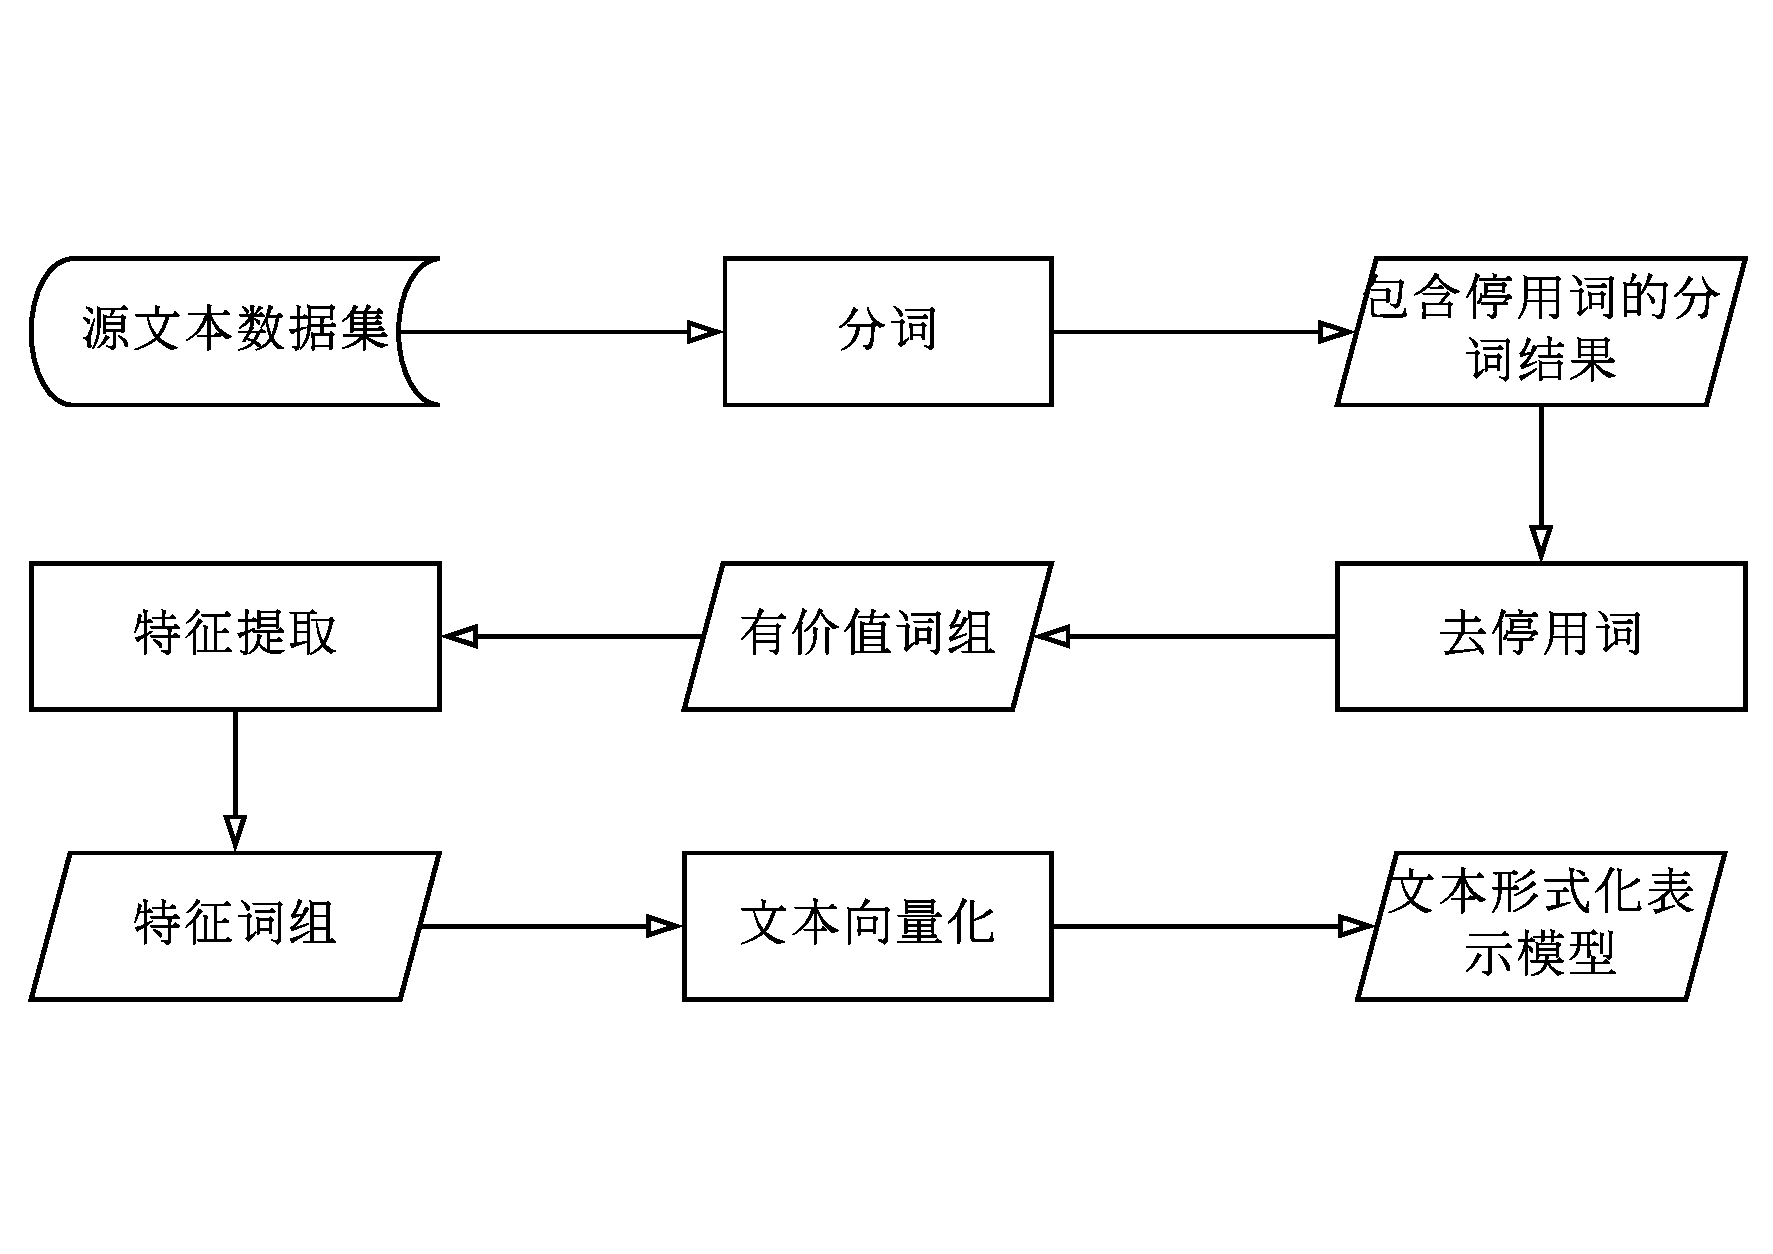
\includegraphics[width=0.8\textwidth]{figure/textPrecess.pdf}
\caption{文本预处理流程}\label{fig:textPrecess}
\end{figure}

\subsubsection{中文分词原理及操作}

在自然语言中,词语一般是最小的具有独立语法或语义的单位.因此,对词的处理自然是文本处理的基础.
对于西方语言,词与词之间由空格分开,非常便于分词.但对于中文,最小的语素是单个文字,词与词之间没有明显的界限区别,所以如何进行分词是中文文本处理首先要解决的一项关键技术.中文分词的任务就是让计算机能按正确的意思识别不同的词.现阶段有的分词有三种方法:基于字符串匹配、基于理解和基于统计的分词方法。

\textbf{基于字符串匹配}的分词方法。基于一定的策略对汉字字符串进行一次分析。匹配大机器字典中的条目。如果在字典中找到字符串,则匹配成功(即识别一个单词)。这些算法的优点是速度快,时间复杂度低,简单有效。但是含糊不清和未列出的单词不能很好地工作。

\textbf{基于理解}的分词方法。基于理解的分词是基于人类对句子理解的计算机模拟,达到识别单词的效果。其基本思想是在使用句法信息的同时进行句法和语义分析。和语义信息处理歧义。它通常由三部分组成:分词子系统、句法子系统和总控部。在总控部的调配下,分词子系统可以得到词和句子的句法语义信息。判断分词的歧义性,即理解句子的过程。这种分词方法需要大量的语言知识和信息。由于汉语知识的广泛性和复杂性,很难将各种语言信息转化为机器该系统可以直接读取的语言。所以现阶段基于理解的分词系统依然不能达到很实用的地步。

\textbf{基于统计}的分词方法。该方法是基于给定大量已分词的文本为前提的。之后,利用统计机器学习模型学习分词的规则(称为训练),从而实现对未知文本的切分。例如最大概率分割法和最大熵分割法。随着大型语料库建立、统计机器学习方法研究和发展的基础上,基于统计的中文分词方法逐渐成为主流方法。在实际应用中,该系统采用分词词典进行字符串匹配和分词。该方法对一些新词进行识别,即将字符串频率统计与字符串匹配相结合,发挥匹配分割的速度。它具有快速、高效的优点,并利用无词典分割和上下文的优点自动识别新词和消除歧义。
主要的统计模型有:N元文法模型(N-gram),隐马尔可夫模型(Hidden Markov Model ,HMM),最大熵模型(ME),条件随机场模型(Conditional Random Fields,CRF)等。


本研究采用Jieba分词工具对评论进行分词,这个工具是使用人数最多的python中文分词库,且支持三种模式:

(1)精确模式:试图将需要分析的句子进行准确的分割,这种方式适应于文本分析;

(2)全模式:把需要解析的句子中所有的可以组成词的词语都找出来, 这样做虽然速度会非常的快,但是不能解决歧义这一问题;

(3)搜索引擎模式:在精确模式的基础之上,通过对长词再次进行分割,提高准确率,这种方式非常适合用于搜索引擎分词。

Jieba分词时主要采用如下算法进行分词:

(1)基于前缀词典实现的高效的词图扫描算法,生成句子中汉字所有可能成词的情况所构成的有向无环图 (DAG);

(2)采用了动态规划的方法查找最大概率路径, 从而找出基于词频的最大切割组合;

(3)对于未登录词,采用基于汉字成词能力的隐马尔可夫模型,之后采用Viterbi算法进行搜索计算;

(4)使用Viterbi算法进行词性的标注;

(5)使用textrank和tf-idf模型得到关键词;

Jieba分词操作示例如图~\ref{fig:Jieba} 所示。
\begin{figure}
  \centering
  \includegraphics[width=0.8\textwidth]{figure/jieba.png}
\caption{Jieba分词操作示例}\label{fig:Jieba}
\end{figure}

\subsubsection{停用词去除}

停止词是一种语言中最常见的词。 这些非常普通的词可以从句子中排除而不改变该句子的含义。 在正常计算程序中处理自然语言数据或文本之前或之后,需要清除停用词。为了给定的目的,可以选择任何组词作为停用词。  这些停用词都是人工输入、非自动化生成的,这些生成后的停用词收集起来会被制作成一个停用词表。

停用词是广泛存在的,甚至是过于频繁的一些单词。比如中文的“我”、“的”之类词几乎在每个文档上均会出现,查询这样的词搜索引擎就无法保证能够给出真正相关的搜索结果,难以缩小搜索范围以提高搜索结果的准确性,同时还会降低搜索的效率。文本中出现频率很高,但实际意义又不大的词。这一类主要包括了语气助词、副词、介词、连词等,通常自身并无明确意义,只有将其放入一个完整的句子中才有一定作用的词语。如常见的“的”、“在”、“和”、“接着”之类。在网页内容中适当地减少停用词出现的频率,可以有效地帮助我们提高关键词密度,有利于提高我们后续分析的精确度。

本次研究一共融合了三个非常丰富的停用词表,生成了$1926$个停用词。该停用词表是已知停用词表中最全的。我们将用此作为后续处理文本数据的停用词删除依据,该停用词样表如图~\ref{fig:stopWorld}所示。

\begin{figure}
  \centering
  \includegraphics[width=0.8\textwidth]{figure/stopworld.png}
\caption{停用词示例}\label{fig:stopWorld}
\end{figure}

\subsubsection{特征词提取方法}~\label{subsec:feature}
文本特征提取方法常用的文本特征自动抽取方法主要有以下几种:词袋模型、N-gram 模型、TF-IDF。

\subsubsection*{(1) 词袋模型}

词袋模型(Bag of words model)是自然语言处理领域中的一种文本特征提取模型。在词袋模型中文本被看作是无序词语的集合,不考虑单词出现的顺序、语法和句法等要素,文档中每个词语的出现都是相互独立的,不依赖于其他词出现与否。
词袋模型首先把语料中的所有词提取出来并进行排序操作,并将所有这些词语构成一个可以用于查找的词典,每一个词都拥有一个代表其在词典中的位置的序号,把这个序号作为作为该词在特征空间中的维度。然后给定一段文本,一个词如果在其中出现一次,就为代表该词的那个维度上加1。

词袋模型假设文本中的词互相独立,并且不考虑词序信息,这让词袋模型便于计算,使其变得简单且高效。但这种简单的表示方法引入了太多重复无用的信息。当文本量较大的时候,由这些文本构造的词典规模也会非常庞大,而用词袋模型表示的向量的维度空间是与词典规模一致的,这导致很容易出现维数灾难问题,即特征向量的维数过大,并且在该向量中大多数维度值都为0,使特征向量非常稀疏。词袋模型由于并没有考虑词语在文本中出现的顺序信息,使得词袋模型不能捕获词与词之间通过语序表达出来的信息。

\subsubsection*{(2) N-gram模型}

N-gram模型是语言模型(Languagemodel)的一种,一般使用N-gram模型是为了预测给定的一个词语序列后出现某个词语的概率。因为N-gram模型简洁有效的特性,其在自然语言处理领域中的应用非常广泛。

N-gram模型是马尔科夫模型的简化版本,马尔科夫模型的核心思想是一个词语出现的概率由它之前的词语决定。在实际使用中,如果考虑之前出现的全部词语会使计算量变得非常大,因此进行简化提出了N-gram模型。N-gram模型假设词语的出现只与它之前的n个词语有关联,而与其他词无关。

N-gram模型特征的表现形式是连续出现的n元词语序列,每一个不同的n元词语序列作为特征的一个维度。与词袋模型提取特征的方式类似,N-gram模型首先统计出所有不同的n元词语序列,把它们按规定的顺序放入词典中以供查询,把每个词语序列在词典的序号作为它们在特征向量空间中的维度。

因为N-gram模型把连续出现的n元词语序列作为一个特征维度,而随着n的值的增大,不同的n元词语序列的个数会呈几何倍数的增长。所以在实际使用中,n一般取值为2 或3。由于N-gram模型能够在一定程度上捕获词语之间的联系信息,其在文本情感分析中的应用也较为频繁。如Blitzer等人使用二元文法特征对特定领域的文本的情感极性进行分析,Cui等人进行的多种特征对比实验结果表明,以二元文法和三元文法作为特征对情感分析的性能有一定的提升作用。Bespalov等人为了进一步减少提取N-gram特征时的计算量,使用隐 N-gram 模型进行特征的提取。

\subsubsection*{(3) TF-IDF}

TF-IDF用于度量
一个词语在一个语料库中某个文档的重要程度。
其最主要的想法是:如果一个词语在一篇文档中高频次的出现,即出现次数多,但是这个词语在其他的文档里出现次数稀少,那么就可以说该词语对于该文档来说具有非常重要的作用,那么这个词就适合作为文本分类的特征。
TF-IDF的计算如公式~\ref{eq:Tf-idf} 所示:
\begin{equation}\label{eq:Tf-idf}
{TF-IDF}_i = {TF}_i \cdot \log(\frac{N}{{DF}_i})
\end{equation}

其中 ${TF}_i$ 表示该词出现的频率,表示在给定的文档词语 $W_i$ 出现的次数:$\log(\frac{N}{DF_i})$ 为反向文档频率,$N$ 为该语料库中总的文档数目,$DF_i$ 表示语料库中包含该词语的文档数目。 $TF_i$ 的计算公式如下公式~\ref{eq:tf} 所示:
\begin{equation}\label{eq:tf}
TF_i = \frac{n_i}{\sum_{k}n_k}
\end{equation}

其中 $n_i$ 表示词语 $w_i$ 在目标文档中的出现次数,$\sum_{k}n_k$是所有词语在文档中的出现频数的总和。因为$TF-IDF$主要用于表达一个词语对某篇文档的重要程度,并不一定能够包含情感信息,所以$TFI-DF$一般用于文档级别的情感分析,需要注意的是仅仅使用$TF-IDF$特征来训练情感分析模型并不足以得到很好的效果。

\subsubsection{文本向量化表示}

文本经过分词等预处理后,还需要对其进行数学建模,从而方便计算机进行计算.目前最常用的是向量空间模型(vector space model,简称VSM.VSM 的基本方法是用特征空间中一组正交的特征词向量表示文本,其中每个不同的词条就作为特征空间中独立的一个维度.采用方法不同得到的向量空间及结果也不同。

例如有两个文档:
\begin{enumerate}
  \item 价格、质量、售后都很满意。
  \item 这件衣服价格实惠,质量也不错。
\end{enumerate}
采用~\ref{subsec:feature} 介绍的词袋模型,
将这两个文本文档中的所有词提取出来,可构造的词典如下:
Dictionary=\{1:“价格”,2:“质量”,3:“售后”,4:“都”,5:“很”,6:“满意”,7:“这件”,8:“衣服”,9:“实惠”,10:“也”,11:“不错”\}。
这个词典一共包含11个不同的词语,利用该词典的索引号,上面两个文档都能用一个11维的向量表示:

\begin{enumerate}
  \item $\left[1, 1, 1, 1, 1, 1, 0, 0, 0, 0, 0 \right]$
  \item $\left[1, 1, 0, 0, 0, 0, 1, 1, 1, 1, 1 \right]$
\end{enumerate}

 采用N-gram模型:
 以“我讨厌吃香蕉”作为例子,如果设n为2,则可以成为序列的词组就有“我讨厌”、“讨厌吃”、“香蕉”,可以假设这些词组在词典中的位置分别为1、4、6,将这几个词组分别作为特征在的向量空间中的一个维度,最后这段文本的特征向量表示为:$\left[1, 0, 0, 1, 0, 1\right]$。

\subsection{情感分析}

目前对文本进行情感分析所用的技术按照类别划分大体上可以分为三类:一类是基于情感词典的文本情感分析方法、一类是基于机器学习的文本情感分析方法以及基于深度习的文本情感分析方法。前两类技术发展较早,都已经较为成熟,基于情感词典的文本情感分析方法的主要思想是把构建好的情感词典作为主要的外部资源,结合定义的规则对文本进行情感分类;基于机器学习的文本情感分析技术主要分为两个步骤,首先提取出文本的特征,然后根据特征训练一个合适的情感分类器,最后使用该分类器进行情感分类。

\subsubsection{基于数据字典的情感分析}

基于情感词典的文本情感分析相关方法最早被用来进行文本的情感分析的。这类方法首先需要有情感词典等外部资源作为基础才能发挥作用,然后对分析文本进行情感词的识别,同时使用语法解析器对文本的语法结构进行解析,最后通过相关规则计算出文本的情感倾向,这样才能实现文本情感分类。
精确而全面的情感词典,可以对情感分析的性能起到很大提升作用。情感词典的构造方法可以分为手工构建和自动构建两种,手工构建的方法通过人工收集和浏览大量的相关语料或者借助现有的情感词典,人工抽取出具有情感倾向的词语,并对其情感极性或情感强度进行标注整合,从而完成情感词典的构建。
国外的情感词典人工构建工作起步较早,使用最为广泛的情感词典是SentiWordNet词典,该词典首先利用WordNet语义关系网把意义相同或相近的词语归集在一起,然后给它们赋予相应的正面情感得分或负面情感得分。GeneralInquirer(GI)被认为是最早的一个情感词典,因为它为每个词的情感极性、情感表达强度和词性等属性分别进行了标注,以便在情感分析中能方便的使用。中文方面,使用最广泛的是知网(HowNet)提供的情感分析词语集,除了情感词之外,HowNet还有一个类似WordNet的词与词之间的语义关系网络。

 \begin{table}
  \centering
  \caption{股票情感词}\label{tb:sentiment}
  \setlength{\tabcolsep}{8mm}{ \begin{tabular}{ccccc}
    \toprule
    % after \\: \hline or \cline{col1-col2} \cline{col3-col4} ...
    正面词 & 负面词 &程度词&否定词&不确定词    \\ \midrule
    佳           &    减少&明显 & 非& 不确定           \\
    优  &  降   &大幅&不&可能                                   \\
    增    &   锐减   &小幅 &并非&或                         \\
    好    &   补跌   &快速 &没 &或是                                               \\
    增长    & 下降    &快 &没  &或将                                              \\
    盈     & 亏损       &适当 &别 &是否                                                \\
    涨    &     赔      &强烈 &无 &有望                                                  \\
    补涨    &    亏        &更 & 未 &疑                                           \\
    赚    & 跌停       &最 &未能&约                                                                \\
    涨停 &   减持  &相当 &没&缘何                                                       \\
    飙升盈利    & 降低   &谨慎 &难 &是否                                          \\\bottomrule
  \end{tabular}}

\end{table}

由于人工构造情感词典需要耗费大量的人力物力,所以学术界更多地聚焦于自动构建情感词典的工作。情感词典的自动构建方法通常是选取一部分词作为情感种子词,基于种子词扩展出一份情感词典,其中最常用的是以点互信息为基础的词语共现法。互信息( mutual information) 是信息论中一种广泛使用的信息度量. 它的研究方法主要是运用数理统计和概率论知识,用来衡量变量之间的依赖程度。点互信息通常被用来衡量两个词之间的独立性,其计算方法如下式所示:
\begin{equation}\label{pmi}
  pmi(x,y) = \log \frac{p(x,y)}{p(x)p(y)}
\end{equation}
其中,$p(x)$和$p(y)$分别表示词$x$和词$y$的概率,$p(x,y)$表示词$x$和词$y$同时出现的概率。$pim(x,y)$表示词$x$和词$y$的同时出现的程度,$pim(x,y)$越大,则表明这两个词同时出现的越频繁,它们的独立性越小。

如果只使用点互信息,我们只能够判断出两个词语之间的共现程度,并不能就此来得出一个词的情感极性。可以通过一个词与情感种子词的紧密程度,来判断该词的情感倾向(Sentimentorientation,SO),其计算方法如公式~\ref{SO} 所示:
\begin{equation}\label{SO}
  SO(w) = p(w,w^{+})-p(w,w^-)
\end{equation}
其中,$w$是待确定情感极性的词$w^{+}$,$w^-$ 和 分别表示正面和负面情感种子词。若SO值大于指定阈值,则其为正面情感词的概率较大,反之则为负面情感词的概率较大,以此来确定词的情感极性。

决定文本情感极性的不仅是文本中的情感词,其中的否定词、程度副词等对其情感倾向也具有很大程度影响,比如情感词前面出现的否定词就能够将其情感进行反转。为了将这些词语的影响考虑到情感计算中来,对这些词语赋予一定的权重,计算情感极性时采用加权求和的方式,如下公式所示:决定文本情感极性的不仅是文本中的情感词,其中的否定词、程度副词等对其情感倾向也具有很大程度影响,比如情感词前面出现的否定词就能够将其情感进行反转。为了将这些词语的影响考虑到情感计算中来,对这些词语赋予一定的权重,计算情感极性时采用加权求和的方式,如下公式~\ref{weight} 所示:
\begin{equation}\label{weight}
  P(S) = \sum_{i=1}^{n}P(w_i)\prod_{j=1}^{m}mod_j
\end{equation}
其中$n$为待分析文本中情感词的个数, 为第$i$个情感词的情感极性的量化值,$m$ 为第$i$个情感词的修饰词的个数, 为第$j$个修饰词的所对应的权重。一般情况下,正面情感词的权重取值大于$0$,负面情感词的权重取值小于$0$,否定修饰词和转折词的权重一般取为$-1$,程度增强修饰词的权值一般大于$1$,程度减弱修饰词的权值则要小于1,最后加权求和计算得到的文本的情感极性值$P(S)$。

按照以上方法进行股票评论文本表示,可以建立一个如表~\ref{tb:sentiment} 所示 的情感词典.情感词典中的词主要通过3 种途径组成:一部分由原始新闻标题新词发现的结果结合人工判断挑选;另一部分根据已有股票领域词典,参考领域专家意见,直接由手工构建;还有一部分则来自“知网HowNet”的情感词库.

基于情感词典的文本情感分析方法由于实施简便和计算速度快等特点,得到了较为广泛的应用,但是这类方法在实际应用中也存在着一些问题,首先是该类方法严重依赖于情感词典的质量,其次是相同的修饰词语出现在不同的语境中时,其修饰效果也会不同,但是这类方法不能很好的解决这个问题,所以引进机器学习的文本情感分析方法。

\subsubsection{基于机器学习方法的情感分析}

基于机器学习的方法是文本情感分析领域的典型方法。该类方法首先从大量标注的样本中提取出表示文本语义信息的特征,然后通过这些特征训练一个合适的文本分类器,最后通过这个训练好的分类器来测试文本的情感类别。基于机器学习的文本分类的方法有很多,其中朴素贝叶斯和支持向量机(SVM)等方法比较成熟。

\subsubsection*{(1)朴素贝叶斯}

朴素贝叶斯(NaïveBayes)是一个简单有效的分类模型,它以贝叶斯定理和特征条件独立性假设为理论基础。在计算过程中,首先利用特征条件独立假设计算得到输入和输出的联合概率分布,当要对输入样本进行预测时,通过贝叶斯定理计算得到所有可能的后验概率,然后从中选择最大那一个作为模型的预测。

设样本的输入空间为 $\mathcal{X}$,其中的向量的维度为 $n$。
输出空间 $P(X,Y)$ 为表示所有的样本类别。
表示的是样本特征 $X$ 与该样本所属类别 $Y=\{c_1,c_2, \dots ,c_k\}$ 的联合概率分布。朴素贝叶斯模型中使用的条件独立性假设可以表述为:在样本所属的类别确定的前提下,该样本的各个维度上的特征 之间是相互独立的。其计算方法如下公式所示:
\begin{align}\label{eq:bayesian}
  P(X=x | Y=c_k) &= P(X^{1}=x^1,\dots,X^{n}=x^n \mid Y=c_k)\\
  &= \prod_{i=1}^{n}P(X^{i}=x^{i} \mid Y=c_k)
\end{align}

在对给定的样本x进行分类时,朴素贝叶斯分类器首先计算出样本属于所有类别的后验概率 ,然后从中选择概率最大的类别 作为对样本类别的预测。这个过程的数学表示如下式所示:
\begin{equation}\label{eq:WeightBayesian}
  \argmax_{c_k}P(Y=c_k)\prod_{i=1}^{n}P(X^{i}=x^{i} \mid Y=c_k)
\end{equation}
朴素贝叶斯模型的实现简单,只需要很少的几个估计参数,对缺失的数据也不敏感,是一种常用文本分类方法。

\subsubsection*{(2)支持向量机}

第二种方法是支持向量机,它也可以在更一致的基础上胜过朴素贝叶斯。这种方法是一种“最大间隔”方法,与使用像朴素贝叶斯和最大熵这样的正确分类概率相反。这种方法是一个双重优化问题,其目标是通过如式~\ref{eq:svm}
的优化来最大化与指定超平面的距离:
\begin{equation}\label{eq:svm}
  \vec{w} \coloneqq \sum_{j}\alpha_{j}c_{j}\vec{d}_{j} \quad \alpha_{j}  \leq  0
\end{equation}

如果$\alpha$是正数,那么文档向量被认为是一个支持向量,因为它有助于解决方案,即文档所处的超平面的哪一侧,从而确定情感分类。

\subsubsection{评论情感分析结果}~\label{subsec:sentiment_result}

利用上述方法分别对于已存储的评论信息进行情感分析,得到每个股票一段时间内的评论的情感倾向。之后以日为单位对评论进行整合,整合策略为一日内积极和消极评论数的众数,若这一日中积极评论占多数,则该日的情感倾向为积极,反之亦然。
基于这样的策略我们得到如图~\ref{fig:emotion} 的情感倾向结果。
\begin{figure}
  \centering
  \captionsetup{justification=centering,margin=2cm}
  \includegraphics[width=0.7\textwidth]{figure/emotion.png}
\caption{情感倾向结果}
\label{fig:emotion}
\end{figure}

\subsection{互信息}

在信息理论开始不久之后\upcite{hockett1953mathematical},现在被称为“互信息”的量被认为是量化任意依赖性问题的原则性解决方案。如果有足够的数据来重构联合概率分布$p(x,y)$,那么可以计算相应的互信息$I(x,y)$。当且仅当$x$和$y$是独立的,这个数量是0; 否则它的值大于0,较大的值对应于较强的依赖性。这些值有一个基本含义:$I(x,Y)$ 是信息量 - 一个变量的值揭示另一个变量的值。而且,可以在任何两种类型的随机变量(实数,多维向量,定性类别等)之间计算信息,
并且$x$和$y$不需要是相同的变量类型。互信息也有一个自然泛化,称为多信息,它量化了三个或更多变量之间的依赖关系。

考虑两个实际连续的随机变量$x$和$y$,从联合概率分布$p(x,y)$得出。 这些变量之间的互信息被定义为~\ref{eq:mi}:

\begin{equation}\label{eq:mi}
  I(x,y) = \int p(x,y)\log_{2}\frac{p(x,y)}{p(x)p(y)} dx dy
\end{equation}

其中$p(x)$和$p(x)$是 $p(x,y)$的边际分布。如此定义下来,互信息具有许多重要的性质。$I(x,y)$ 是非负的,$I(x,y) = 0$仅在$p(x,y)= p(x)p(y)$ 时出现。 因此,当$x$和$y$表现出任何相互依赖性时,互信息将大于$0$,而不管这种依赖性有多么非线性。 而且相互依赖性越强$I(x,y)$ 越大.在$y$是$x$的确定函数的取极限下,$I(x,y) = \infty$。

但是,从有限数据中准确估计互信息是非常重要的。 困难在于从$N$个数据点的有限样本估计联合分布$p(x,y)$。 最简单的方法是“分箱”数据 - 在x-y散点图上叠加一个矩形网格,然后将每个连续x值(或y值)分配给它所在的列仓X(或行仓Y)。 然后可以利用式~\ref{eq:mi_dis}从所得到的离散化联合分布$p(x,y)$中估计互信息:
\begin{equation}\label{eq:mi_dis}
  I(x,y) \approx I(X,Y) = \sum_{X,Y}\log_{2}\frac{p(X,Y)}{P(X)p(Y)}
\end{equation}

其中$p(X,Y)$是落入箱$(X,Y)$的分箱数据的分数。 依赖这种简单分箱程序的相互信息估计被称为“天真”估计。 这种天真估计的问题是他们系统地高估了I(x,y)。 这一直被认为是一个问题,并且一直致力于提供其他方法来精确估计互信息。 但是,这个估计问题随着$N$ 变大而变得更容易。 在大数据极限$(N\to \infty)$中,联合分布$p(x,y)$ 可以确定为任意精度,因此$I(x,y)$可被计算出来。


人们早已认识到,互信息能够量化依赖关系的强度,而不必考虑这些依赖关系的特定功能形式. 然而,互信息并不符合公平观念,但将互信息的特定估计归一化为一个他们称之为“最大信息系数”(MIC)的新统计量能够恢复公平性。

\subsection{最大信息系数}

最大信息系数(MIC)是衡量两个变量X和Y之间线性或非线性关联强度的一个度量\upcite{reshef2011detecting}
最大信息系数使用分箱作为在连续随机变量上应用互信息的手段。 长期以来,分档已被用作将互信息应用于连续分布的一种方式; 此外,MIC还提供了一种方法,用于选择垃圾箱数量并在许多可能的网格中选择最大值。

Reshef等人\upcite{reshef2011detecting}在不同关系的数据和加入不同程度的噪音数据的情况下做了如图~\ref{fig:mic}所示的结果。
从中可以看到MIC不仅可以找出两个变量之间线性关系,而且可以衡量非线性关系。
更进一步,MIC的衡量方法对于噪音的敏感度低,因此,本研究选择MIC作为衡量股民评论情感和股票趋势走向的度量。
\begin{figure}
  \centering
  \includegraphics[width=0.8\textwidth]{figure/mic.png}
\caption{MIC 测试实例}
\label{fig:mic}
\end{figure}


\subsection{相关性度量及结论}~\label{subsec:sum}

本研究中利用式~\ref{eq:mic}在这$N$个数据点(x,y)对上定义MIC\upcite{reshef2011detecting}。
\begin{equation}\label{eq:mic}
  MIC(x,y) = \max_{ \left| X \right| \left| Y \right|<B}\frac{I(X,Y)}{\log_2 (\min( \left| X \right|, \left| Y \right|))}
\end{equation}

具体操作如下,首先将每个数据点$(x,y)$分配给箱$(X,Y)$的箱装方案。 然后利用式~\ref{eq:mi_dis}根据频率表  $p(X,Y)$计算简单的互信息估计 $I(X,Y)$。  之后除以$X$箱的记录数(表示为$|X|$)或Y箱($|Y|$)其中较小者的$\log$值。 当然,得到的值将取决于两个维度中的箱的数量以及箱边界的绘制位置,其中分箱的总数量$|X||Y|$小于某个数字$B$.
事实上,$0 \leq I(x,y) \leq \log_{2}(\min(|X|,|Y|)$,这意味着MIC将始终落在$0$和$1$之间。

但是,这种标准化方案并不能防止过度拟合。 例如,考虑包含偶数个数据点$N$的数据集,其中所有$x$和$y$值都是不同的。 在这种情况下,可以将观察到的$x$值平均分配到两个$X$区间,同时将一个$y$值分配到$N$个不同的$Y$区间中的每一个中。 这产生$MIC(x, y) = 1$,而不管数据中的实际$x$和$y$值如何。 对满足$|X ||Y|$的分箱方案的限制 在等式~\ref{eq:mic}规避了这种弊病; 因此我们采用Reshef等人\upcite{reshef2011detecting}主张使用的$B = 0.6N$。虽然这些选择的数学基本原理并不清楚。

经过上述方法,可计算出处将情感态度作$X$。与第二日的价格因变量$Y$的$MIC$值为$0.73$。虽然$0.73$看起来值并不高,但考虑到影响股票价格因素大多样性,在的大样本的情况下,$0.73$这样的关联程度足以说明由于两个变量之间存在着相关性。因此,居于此,可以得出消费者评论的情绪价值与股票价格之间存在统计上显着的关系。人们分享他们对于股票的态度会以多种方式影响该股票的走势。


\section{总结和展望}~\label{总结}

本章介绍了这项研究的主要发现,包括主要影响。 将讨论管理和理论方面的贡献。 这项研究提供了洞察情绪分析的应用作为股票价格的关联。 任何可能适用于本研究的限制都将被详细描述。 最后,将讨论未来研究的想法。

\subsection{总结}

\subsection{待研究问题}~\label{待研究问题}


%============= 参考文献 =====================
\newpage
\addcontentsline{toc}{section}{参考文献}
\nocite{*}
%\bibliographystyle{plain}
\bibliography{bibfile}
%\clearpage
%=============  致谢  ======================
\section*{致谢}
\addcontentsline{toc}{section}{致谢}

本次论文是在我的导师孔劼孔老师的亲切关心和悉心指导下完成的。从论文课题的选择到最终完成,孔老师都始终给予我细心的指导和不懈的支持。感谢孔老师在大学四年中对我的帮助和指导!您当初的指导,为我开启了人工智能方向的学习的大门。 在此谨向您致以诚挚的谢意!

感谢李刚教授,李刚教授以严谨的科研态度和孜孜不倦的教诲将我引入人工智能方向的研究及学习。没有老师的教导,我很难在本科阶段就开始到人工智能方向的科研训练,并坚定继续学习和科学研究的决心!再次感谢李老师!

感谢我的舍友刘楠、赵小建、和努尔阿力木以及我所有的同学!感谢你们在大学四年中对我的的理解和帮助! 感谢你们在我烦恼时,倾听我的忧愁以及带给我的所有的欢乐!

感谢实验室的师兄师姐及一起接受科研训练的同门,特别是王聪颖在大学四年中对我科研及学习方面的帮助,没有你们的帮助、鼓励和支持,我很难在学习和科研的道路上坚持下来!

特别的,我要感谢父母的鼓励和支持。在我的十几年求学历程里,是父母辛勤的劳作和无私的付出,为我创造良好的学习条件,我才能顺利完成完成学业,感激父母一直以来对我的抚养与培育!

感谢所有在我大学四年间出现的可爱的人们,你们构成了我大学所有的美好回忆,这将会成为我终生的宝贵财富!



%=============  附录 ======================
%\section*{附录}
\addcontentsline{toc}{section}{附录}
在本次论文的写的过程,会用到以下算法,现我将简要将这些算法介绍。

\subsection*{附录1  算法类似性}

(1)决策树学习:根据数据的属性采用树状结构建立决策模型。决策树模型常常用来解决分类和回归问题。常见的算法包括 CART (Classification And Regression Tree)、ID3、C4.5、随机森林 (Random Forest) 等。

(2)回归算法:试图采用对误差的衡量来探索变量之间的关系的一类算法。常见的回归算法包括最小二乘法 (Least Square)、逻辑回归 (Logistic Regression)、逐步式回归 (Stepwise Regression) 等。

(3)聚类算法:通常按照中心点或者分层的方式对输入数据进行归并。所有的聚类算法都试图找到数据的内在结构,以便按照最大的共同点将数据进行归类。常见的聚类算法包括 K-Means 算法以及期望最大化算法 (Expectation Maximization) 等。

(4)人工神经网络:模拟生物神经网络,是一类模式匹配算法。通常用于解决分类和回归问题。人工神经网络算法包括感知器神经网络 (Perceptron Neural Network) 、反向传递 (Back Propagation) 和深度学习等。

\newpage

\subsection*{附录2   决策树模型评估}

建立了决策树模型后需要给出该模型的评估值,这样才可以来判断模型的优劣。学习算法模型使用训练集 (training set) 建立模型,使用校验集 (test set) 来评估模型。本文通过评估指标和评估方法来评估决策树模型。 评估指标有分类准确度、召回率、虚警率和精确度等。而这些指标都是基于混淆矩阵 (confusion matrix) 进行计算的。

混淆矩阵是用来评价监督式学习模型的精确性,矩阵的每一列代表一个类的实例预测,而每一行表示一个实际的类的实例。以二类分类问题为例,如下表所示:

\begin{table}[thbp]\footnotesize
	\caption{混淆矩阵}
	\begin{center}
		\begin{tabular}{cc|clc}
			\hline	&预测的类\\
			  实际的类& & 类=1 & 类=0  \\
			\hline &类=1 & TP & FN &P\\ 	
			\hline &类=0 & FP & TN&N \\
			\hline
		\end{tabular}
	\end{center}
\end{table}


P (Positive Sample):正例的样本数量。

N(Negative Sample):负例的样本数量。

TP(True Positive):正确预测到的正例的数量。

FP(False Positive):把负例预测成正例的数量。

FN(False Negative):把正例预测成负例的数量。

TN(True Negative):正确预测到的负例的数量。

根据混淆矩阵可以得到评价分类模型的指标有以下几种。

分类准确度,就是正负样本分别被正确分类的概率,计算公式为:

\begin{equation}
Accuracy=\frac{TP+TN}{P+N}
\end{equation}

召回率,就是正样本被识别出的概率,计算公式为:

\begin{equation}
Recall=\frac{TP}{P}
\end{equation}

虚警率,就是负样本被错误分为正样本的概率,计算公式为:

\begin{equation}
FPrate=\frac{FP}{N}
\end{equation}

精确度,就是分类结果为正样本的情况真实性程度,计算公式为:

\begin{equation}
Precision=\frac{TP}{TP+FP}
\end{equation}

评估方法有保留法、随机二次抽样、交叉验证和自助法等。

保留法 (holdout) 是评估分类模型性能的最基本的一种方法。将被标记的原始数据集分成训练集和检验集两份,训练集用于训练分类模型,检验集用于评估分类模型性能。但此方法不适用样本较小的情况,模型可能高度依赖训练集和检验集的构成。

随机二次抽样 (random subsampling) 是指多次重复使用保留方法来改进分类器评估方法。同样此方法也不适用训练集数量不足的情况,而且也可能造成有些数据未被用于训练集。

交叉验证 (cross-validation) 是指把数据分成数量相同的 k 份,每次使用数据进行分类时,选择其中一份作为检验集,剩下的 k-1 份为训练集,重复 k 次,正好使得每一份数据都被用于一次检验集 k-1 次训练集。该方法的优点是尽可能多的数据作为训练集数据,每一次训练集数据和检验集数据都是相互独立的,并且完全覆盖了整个数据集。也存在一个缺点,就是分类模型运行了 K 次,计算开销较大。

自助法 (bootstrap) 是指在其方法中,训练集数据采用的是有放回的抽样,即已经选取为训练集的数据又被放回原来的数据集中,使得该数据有机会能被再一次抽取。用于样本数不多的情况下,效果很好。
\appendix 
\end{document}
%%%%%%%%%% 结束 %%%%%%%%%%
